\addtocontents{toc}{\protect\newpage}
% {Youssouph Cissokho}

\section{Anomalies in High-Dimensional Datasets}\label{Section:4}
%
%
% 
Anomaly detection is a broad field of study that has been applied to a large number of areas. Nowadays, many real datasets are very large; in some scenarios, the observations may contain \textbf{hundreds or thousands of features} (or dimensions).
\par Many classical methods use proximity (distance) concepts for anomaly detection (see Section 2 for a sample of such methods) and can only be applied in cases where the sample size $n$ is larger than the dimension $p$ ($n>p$). 
\newl
The management of \textbf{high-dimensional data} ($n<p$) offers specific difficulties: indeed, in such spaces observations are often \textbf{isolated} and \textbf{scattered} (or sparse) and the notion of proximity fails to maintain its relevance. 
\par In that case, the notion of defining significant outliers is much more complex and not obvious: many conventional methods of detecting outliers are simply not efficient in the high-dimensional context, due to this \textbf{curse of dimensionality}.\newl
The remainder of this section is organized as follows: first, an attempt is made to define the concept and the challenges; then, anomaly detection techniques are discussed; finally, we end with a detailed description of ensembles and subspace methods. Our approach mainly follows those found in \cite{A1,A8,A10,A14,Aurore}.
%
%
\subsection{Definitions and Challenges}

As we have seen previously, an anomalous observation is one that deviates or behaves differently from other the observations in the dataset, which makes us suspect that it was generated by some other mechanism \cite{A1}; such an observation would, of course, be considered to be irregular. 

%
The challenges of anomaly and outlier detection  in high-dimensional data lie in the facts that:
\begin{itemize}[noitemsep]
\item the notion of distance fails to retain its relevance due to the curse of dimensionality (whence ``the problem of detecting outliers is like finding a needle in a haystack'' \cite{A14});
\item every point in such datasets has a tendency to be an outlier, and 
\item datasets become more sparse as the dimension of the feature space increases.
\end{itemize}

\noindent The authors of \cite{AYU} consider that in order to deal properly with large datasets, detection methods should:
\begin{enumerate}[noitemsep]
\item allow for effective management of sparse data issues;
\item provide interpretability of the discrepancies (i.e.\@ how the behaviour of such observations is different);
\item allow anomaly measurements to be compared, and 
\item consider the local data behaviour to determine whether an observation is abnormal or not.
\end{enumerate}
%
\subsection{Projection-Based Methods}
Nowadays, it is common to deal with very large data sets known as HDLSS (\textbf{high dimension, low sample size}), which can contain hundreds of variables (or even more). \par As a result,  the curse of dimensionality affects the efficiency of conventional anomaly/outlier detection methods.\newl One solution to this problem is to \textbf{reduce the dimensionality} of the dataset while preserving its essential characteristics. Such projecion-based methods \begin{itemize}[noitemsep]\item principal component analysis, \item linear discriminant analysis, \item feature selection, etc. \end{itemize} In this section, We provide details on one such method: PCA.
\subsubsection*{Principal Components Analysis}
%
\textbf{Principal components analysis} (PCA) aims to find a representation of the original dataset in a lower-dimensional subspace (such as a line or a plane)  containing the greatest possible variation. 

PCA corresponds to an orthogonal linear transformation of the data into a new coordinate system, such that the largest variance resulting from a scalar projection of the data is on the first coordinate (the \textbf{first principal component}), the second largest variance on the second coordinate, and so forth.\newl PCA is used in various contexts:
\begin{itemize}[noitemsep]
    \item as a dimension reduction method used during the data pre-processing step;
    \item as a data visualization aid, and, in the scenario of interest for this report, 
    \item as an anomaly and outlier detection method.
\end{itemize}
Let the dataset be represented by a numerical, centered, and scaled $n\times p$ matrix $\textbf{X}=[\textbf{X}_1,\cdots,\textbf{X}_p]$ with $n$ observations (number of rows) and $p$ features (number of columns). The \textbf{principal components} can be written as linear combinations of the variables 
\begin{align*}
\textbf{Y}_i=\ell^{\!\top}_i\textbf{X}=\ell_{1,i}\textbf{X}_1+\cdots+\ell_{p,i}\textbf{X}_p;\quad i=1,\cdots,k,
\end{align*}
with $k\leq p$, yielding the largest variance subjet to the constraint $\|\ell_i\|=1$ (where $\|\cdot\| $ represents the Euclidean norm). We can thus deduce that  
\begin{align*}
\operatorname{Var}\left(Y_{i}\right) &=\operatorname{Var}\left(\ell_{i}^{\!\top} \boldsymbol{X}\right)=\ell_{i}^{\!\top} \boldsymbol{\Sigma} \ell_{i} \,,\\ 
\operatorname{Cov}\left(Y_{i}, Y_{k}\right) &=\operatorname{Cov}\left(\ell_{i}^{\!\top} \boldsymbol{X}, \ell_{k}^{\!\top} \boldsymbol{X}\right)=\ell_{i}^{\!\top} \boldsymbol{\Sigma} \ell_{k}\, .
\end{align*}
In other words, PCA finds the \textbf{loadings vector} $\ell_{1}$ which maximizes the variance of $Y_1$, i.e. 
\begin{align*}
\mathbf{\ell}_{1}&=\underset{\|\mathbf{\ell_1}\|=1}{\arg \max }\left\{\ell^{\!\top}_1\mathbf{X}^{\!\top} \mathbf{X} \ell_1\right\},
\end{align*}
then the loadings vector $\ell_2$ (not correlated with $\ell_1$) which maximizes the variance of $Y_2$, i.e.   
\begin{align*}
\mathbf{\ell}_{2}& =\underset{\|\mathbf{\ell_2}\|=1,\; \ell_{1}^{\!\top}\ell_{2} =0}{\arg \max }\left\{\ell^{\!\top}_2\mathbf{X}^{\!\top} \mathbf{X} \ell_2\right\}.
\end{align*}
Similarly, the loadings vector $\ell_k$ is not correlated with any of the $\ell_i$, $i<k$, and maximizes the variance of $Y_k$, i.e.
\begin{align}
\mathbf{\ell}_k=\underset{\substack{\|\ell_k\|=1,\\ \;\ell_{i}^{\!\top}\ell_k=0,\;\forall\;i<k}}{\arg \max} \left\{\ell^{\!\top}_k\mathbf{X}^{\!\top} \mathbf{X} \ell_k\right\}.\label{eq1}
\end{align}
We solve \eqref{eq1} for all  $i<k$ through the Lagrangian
\begin{align*}
L=\ell^{\!\top}_k\mathbf{X}^{\!\top} \mathbf{X} \ell_k-\lambda_k(\ell^{\!\top}_k\ell_k-1)-w\ell_{i}^{\!\top}\ell_k.
\end{align*}
The critical points are found by differentiating with respect to each of the entries of $\ell_k$, $\lambda_k$ and $w$, and setting the result to 0. Simplifying, we obtain  
\begin{align*}
\mathbf{X}^{\!\top} \mathbf{X} \ell_k&=\lambda_k\ell_k\\
\ell^{\!\top}_k\ell_k&=1 \quad\text{et}\quad\ell^{\!\top}_k\ell_i=0,\quad\text{for all}\; i<k.
\end{align*}
The loadings vector $\ell_k$ is thus the \textbf{eigenvector} of the design matrix $\mathbf{X}^{\!\top} \mathbf{X}$ associated to the $k$th largest eigenvalue. \newl
%\begin{lemma} Les $k$ ($k<p$ composantes principales donnant la plus grande variance maximale sont données par les $k$ vecteurs propres associés aux $k$ plus grandes valeurs propres de $\mathbf{X}^{\!\top} \mathbf{X}$.\end{lemma}
The \textbf{proportion of the variance which can be explained} by the PCA can be calculated by first noting that 
\begin{align*}
\sum_{i=1}^{p}\operatorname{Var}\left(Y_{i}\right) &=\sum_{i=1}^{p}\ell_{i}^{\!\top} \boldsymbol{\Sigma} \ell_{i}=\sum_{i=1}^{p}\lambda_i \,.
\end{align*}
Consequently, the proportion of the total variance explained by the $i$th principal component is  
\begin{align*}
0\leq \frac{\lambda_i}{\sum_{i=1}^{p}\lambda_i }\leq 1
\end{align*}
The quality of the PCA results is strongly dependent on the number of retained principal components, that is, on the dimension $k$ of the subspace on which the observations are projected. There are multiple ways to select the ``right'' $k$ -- we will briefly present two of them. 
\newl The proportion of the total variance explained by the first $k$ principal components is given by  
\begin{align*}
p_k=\frac{\sum_{i=1}^{k} \lambda_i}{\sum_{i=1}^{p}\lambda_i}.
\end{align*}
One approach is to retain $k$ principal components, where $k$ is the smallest value for which  $p_k$ surpasses some pre-established threshold  (often taken between $80\%$ and $90\%$). \newl
The \textbf{scree plot method}, on the other hand, consists in drawing the curve given by the decreasing eigenvalues (the \textbf{scree plot}), and to identify the curve's ``elbows''. These points correspond to principal components for which the variance decreases at a slower rate with added components. If such an elbow exists, we would retain the eigenvalues up to it (and thus,  the corresponding principal components). 
\begin{Example}
PCA is applied on a dataset of genetic expression measurements, for $n=72$ leukemia patients and $p=7128$ genes \cite{Hleukemia}. The scree plot suggests that only one principal component should be retained; the projection on the first 3 principal components is also shown in Figure~\ref{fig0} (on the right). Some R code is given below.
\begin{figure*}[t]
    \centering
     \includegraphics[width=.55\textwidth]{ADOA/Images/screeleuk_\ldoc.png}
    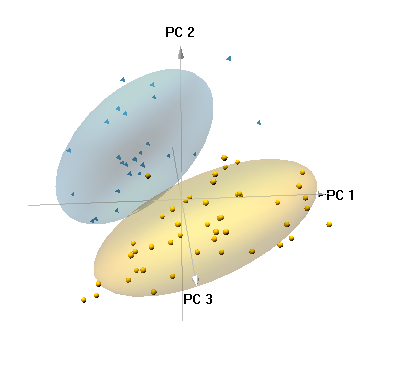
\includegraphics[width=.4\textwidth]{ADOA/Images/3dpcleuk.PNG}
    \caption{Scree plot (left); projection on the first 3 principal components (right).}\hrule
    \label{fig0}
\end{figure*}
\begin{lstlisting}
leukemia.big <- read.csv("http://web.stanford.edu/~hastie/ CASI_files/DATA/leukemia_big.csv")
leukemia.big <- t(leukemia.big)
leukemia.big.scaled <- scale(leukemia.big)
pca.leukemia <- prcomp(leukemia.big.scaled)
plot(pca.leukemia)
pca.leukemia.s <- summary(pca.leukemia) 
plot(pca.leukemia.s$importance[3,])
\end{lstlisting}
\end{Example}
\noindent There are other PCA-associated dimension reduction methods, such as the singular value decomposition, kernel PCA, and so forth; more details are available in \cite{BLMMP}.
\newl What is the link with anomaly and/or outlier detection? Once the dataset has been projected on a lower-dimensional subspace, the curse of dimensionality is mitigated -- it is on the projected data that the traditional detection methods are applied. \par Note, however, that any such reduction necessarily leads to a loss of information, which can affect the accuracy of the detection procedure, especially if the presence/absence of anomalies is not aligned with the dataset's principal components. 

\subsubsection*{Distance-Based Outlier Basis Using Neighbours}
Using PCA for anomaly detection is potentially problematic, however: whether an observation is anomalous or not does not figure in the construction of the principal component basis $\{\text{PC}_1,\ldots,\text{PC}_k\}$ -- there isn't necessarily a correlation between the axes of heightened variance and the presence or absence of anomalies. 
\newl 
The \textbf{distance-based outlier basis using neighbours} algorithm (DOBIN) builds a basis which is better suited for the eventual detection of outlying observations. DOBIN's main idea is to search for nearest neighbours that are in fact relatively distant from one another: 
\begin{enumerate}[noitemsep] 
\item We start by building a space $\mathbf{Y}=\{\mathbf{y}_{\ell}\}$  which contains $M\ll n(n+1)/2$  vectors of the form $$\mathbf{y}_{\ell}=(\mathbf{x}_i -\mathbf{x}_j)\odot (\mathbf{x}_i -\mathbf{x}_j), $$ where $\odot$ is the element-by-element Hadamard multiplication, and for which the $1-$norm  $$\|\mathbf{y}_{\ell}\|_1=(x_{1,1}-x_{2,1})^2+\cdots +(x_{1,p}-x_{2,p})^2 $$ is the square of the distance between $\mathbf{x}_i,\mathbf{x}_j \in\mathbf{X}$ (the selection of each of the $M$ observation pairs is made according to a rather complex procedure which only considers $\mathbf{x}_i$ and $\mathbf{x}_j$ if they are part of one another's $k-$neighbourhood, for $k\in\{k_1,\ldots, k_2\}$); the set $\mathbf{Y}$ thus contains points for which $\|\mathbf{y}_{\ell}\|_1$ is relatively large, which is to say that the observations $\mathbf{x}_i$ are $\mathbf{x}_j$ fairly distant from one another even if they are $k-$neighbours of each other;
\item we next build a basis $\{\eta_1,\ldots,\eta_p\}\subset \mathbb{R}^p$ where each  $\eta_i$ is a unit vector given by a particular linear combination of points in $\mathbf{Y}$; they can be found using a  Gram-Schmidt-like procedure: 
\begin{align*}
\mathbf{y}_{\ell_0}&=\mathbf{y}_{\ell},\quad \ell=1,\ldots, M \\ 
%\eta_1&=\frac{\sum_{\ell=1}^M\mathbf{y}_{\ell}}{\left\|\sum_{\ell=1}^M\mathbf{y}_{\ell}\right\|_2} \\
%\mathbf{y}_{\ell_1}&=\mathbf{y}_{\ell}-\langle\eta_1 \mid \mathbf{y}_{\ell}\rangle,\quad \ell=1,\ldots, M \\ 
%\eta_2&=\frac{\sum_{\ell=1}^M\mathbf{y}_{\ell_1}}{\left\|\sum_{\ell=1}^M\mathbf{y}_{\ell_1}\right\|_2} \\ 
\mathbf{y}_{\ell_{b-1}}&=\mathbf{y}_{\ell_{b-2}}-\langle\eta_{b-1} \mid \mathbf{y}_{\ell_{b-2}}\rangle,\quad \ell=1,\ldots, M \\ 
\eta_b&=\frac{\sum_{\ell=1}^M\mathbf{y}_{\ell_{b-1}}}{\left\|\sum_{\ell=1}^M\mathbf{y}_{\ell_{p-1}}\right\|_2},
\end{align*} for $b=1,\ldots,p$,
\item and we tranform the original dataset   $\mathbf{X}$ according to  $\hat{\mathbf{X}}=\mathcal{T}(\mathbf{X})\Theta,$ where $\mathcal{T}(\mathbf{X})$ normalizes each feature of  $\mathbf{X}$ according to a problem-specific scheme  (Min-Max or Median-IQR, say) and $$\Theta=[\eta_1\mid\cdots\mid \eta_p]$$ is a orthogonal $p\times p$ matrix.  
\end{enumerate}
It is on the transformed space (which plays an analogous role to the subspace projection of  $\mathbf{X}$ in PCA) that we apply the various outlier and anomaly detection algorithms.\newl 
The full details contain a fair number of technical complications; the interested reader is invited to consult the original documentation \cite{A6} (note that the algorithm is implemented in R \textit{via} the module \textit{dobin}). 
%
\subsection{Ensembles Methods}
%
%
In the preceding sections, we have described various anomaly detection algorithms whose relative performance varies with the type of data being considered. It's usually impossible to come up with an algorithm that outperforms all the others. \par This is because a particular anomaly detection algorithm may be well adapted to a data set and may be successful in detecting abnormal or outlier observations, but it may not work with other data sets whose characteristics do not match the first data set. \newl The impact of such a mismatch between algorithms can be mitigated by using  \textbf{ensemble methods}, where the results of several algorithms are considered before making a final decision. Such an approach often provides the best results and thus improves the performance of the base anomaly detection algorithms \cite{A10}. 
\newl We will consider two types of ensemble methods:  \textbf{sequential ensembles} (boosting) and \textbf{independent ensembles}, 
\subsection*{Sequential Ensembles}
Sequential ensembles requires a given algorithm (or a set of algorithms) to be applied to a dataset in a sequential manntter, each time on a slightly different dataset derived from the previous step's dataset based on the previous steps' results, and so forth. At each step, the weight associated with each observation is modified according to the preceding results using some ``boosting'' method (such as AdaBoost or XGBoost, for instance). \newl The final result is either some weighted combination of all preceding results, or simply the results output by the last step in the sequence (see Algorithme~\ref{algSeq}). 

The details are out-of-scope for this report, but can be studied in \cite{LB}.

\begin{algorithm}
\SetAlgoLined
\textbf{Inputs:} dataset $D$, base algorithms $A_1,\ldots,A_r$ 

$j=1$\;
\While{stopping criteria are not met}{
	Select an algorithm $A_j$ based on the results from the preceding steps\;
	Create a new dataset $D_j$ from $D$ by modifying the weight of each observation based on the results from the preceding steps\;
	Apply $A_j$ to $D_j$\;
	$j=j+1$\;
}
\textbf{Output:} anomalous observations obtained by weighing the results of all previous steps 
\caption{SequentialEnsemble}\label{algSeq}
\end{algorithm}%\newl
\subsection*{Independent Ensembles}
In an independent ensemble, we instead apply different algorithms (or different instanciations of the same algorithm) to the dataset (or some resampled dataset). \par Choices made at the data and algorithm level
are independent of the results obtained in previous runs (unlike in a sequential ensemble). The results are then combined to obtain more robust outliers (see Algorithm~\ref{algInd}).

\begin{algorithm}[t]
\SetAlgoLined
\textbf{Inputs:} dataset $D$, base algorithms $A_1,\ldots,A_r$ 

$j=1$\;
\While{stopping criteria are not met}{
	Select an algorithm $A_j$\;
	Create a new dataset $D_j$ from $D$ by (potential) re-sampling, but independently of the preceding steps' results\;
	Apply $A_j$ to $D_j$\;
	$j=j+1$\;
}
\textbf{Output:} anomalous observations obtained by combining the results of all previous steps 
\caption{IndependantEnsemble}\label{algInd}
\end{algorithm}
\ \\
\noindent Every base anomaly detection algorithm provides an a\-no\-ma\-ly score (or an abnormal/regular classification) for each observation in $D$; observations with higher scores are considered to be more anomalous, observations with lower scores more normal. \par The results are then combined using a task-specific method in order to provide a more robust classification of anomalous or outlying observations. 
\newl Many such combination techniques used in practice:  \begin{itemize}[noitemsep]
\item \textbf{majority vote}, 
\item \textbf{average}, 
\item \textbf{minimal rank}, etc. \end{itemize}  
Let $\alpha_i(\mathbf{p})$ represent the (normalized) \textbf{anomaly score} of $\mathbf{p}\in D$, according to algorithm $A_i$. If $\alpha_i(\mathbf{p})\approx 0$, it is unlikely that $\mathbf{p}$ is an anomaly according to $A_i$, whereas if $\alpha_i(\mathbf{p})\approx 1$, it is quite likely that $\mathbf{p}$ according to $A_i$. \par The \textbf{rank} of $\mathbf{p}\in D$ according to $A_i$, on the other hand, is denoted by $r_i(\mathbf{p})$: the higher the rank (smaller number), the higher the anomaly score  \textit{vice versa}. In a dataset with  $n$ observations, the rank varies from $1$ to $n$ (ties are allowed). 
\par If the base detection algorithms are $A_1, \ldots, A_m$, the anomaly score and the rank of an observation $\mathbf{p}\in D$ according to the independent ensemble method are, respectively, 
\begin{align*}
\alpha(\mathbf{p})=\frac{1}{m}\sum_{i=1}^{m}\alpha_i(\mathbf{p}) \qquad \text{and}\; \qquad r(\mathbf{p}) =\min_{1\leq i \leq m} \{r_i(\mathbf{p})\}.
\end{align*}
If $n=m=3$, for instance, we could end up with 
\begin{align*}\alpha_{1}\left(\mathbf{p}_{1}\right)&=1.0,\; \alpha_{1}\left(\mathbf{p}_{2}\right)=0.9,\; \alpha_{1}\left(\mathbf{p}_{3}\right)=0.0; \\ 
\alpha_{2}\left(\mathbf{p}_{1}\right)&=1.0,\; \alpha_{2}\left(\mathbf{p}_{2}\right)=0.8,\; \alpha_{2}\left(\mathbf{p}_{3}\right)=0.0;\\
\alpha_{3}\left(\mathbf{p}_{1}\right)&=0.1,\;  \alpha_{3}\left(\mathbf{p}_{2}\right)=1.0,\; \alpha_{3}\left(\mathbf{p}_{3}\right)=0.0.
\end{align*}
Using the mean as the combination techniques, we obtain
\begin{align*}
\alpha\left(\mathbf{p}_{1}\right)&=0.7,\; \alpha\left(\mathbf{p}_{2}\right)=0.9,\; \alpha\left(\mathbf{p}_{3}\right)=0.0,
\end{align*}
whence $$\mathbf{p}_2\succeq \mathbf{p}_1\succeq \mathbf{p}_3,$$ that is, $\mathbf{p}_2$ is more anomalous than $\mathbf{p}_1$, which is itself more anomalous than  $\mathbf{p}_3$ (see the notation introduced on page~\pageref{succeq}). 
\newl 
Using the minimal rank method, we obtain 
\begin{align*}
r_{1}\left(\mathbf{p}_{1}\right)&=1,\; r_{1}\left(\mathbf{p}_{2}\right)=2,\; r_{1}\left(\mathbf{p}_{3}\right)=3;\\ 
r_{2}\left(\mathbf{p}_{1}\right)&=1,\; r_{2}\left(\mathbf{p}_{2}\right)=2,\; r_{2}\left(\mathbf{p}_{3}\right)=3;\\
r_{3}\left(\mathbf{p}_{1}\right)&=2,\; r_{3}\left(\mathbf{p}_{2}\right)=1,\; r_{3}\left(\mathbf{p}_{3}\right)=3,
\end{align*}
from which 
\begin{align*}
r\left(\mathbf{p}_{1}\right)=r\left(\mathbf{p}_{2}\right)=1,\; r \left(\mathbf{p}_{3}\right)=3, 
\end{align*}
whence $\mathbf{p}_1\succeq \mathbf{p}_3$ and $\mathbf{p}_2\succeq \mathbf{p}_3$, but $\mathbf{p}_1$ and  $\mathbf{p}_2$ have the same anomalous levels. 
\newl Evidently, the results depend not only on the data set under consideration and on the base algorithms that are used in the ensemble, but also on how the results are combined. 
\newl In the context of HDLSS data, ensemble methods can sometimes allow the analyst to mitigate some of the effects of the curse of dimensionality by selecting fast base algorithms (which can be run multiple times) and focusing on building robust relative anomaly scores. \par Another suggested  approach is to use a different subset of the original dataset's features at each step, in order to de-correlate the base detection models. 
%
%


%
\subsection{Subspace Methods}
%
%
\textbf{Subspace methods} have been used particularly effectively by analysts for anomaly and outlier detection in high-dimen\-sional data sets \cite{A8,A13,A14}; it is often easier to find the sought-after observations by exploring  lower-dimensional subspaces (rather than the original set). \par There is thus an intrinsic interest in exploring subspaces in their own right  \cite{A1,Aurore}. This approach eliminates \textbf{additive noise effects} often found in high dimensional spaces and leads to more robust outliers (that is, outliers which are identified as such even when using different methods). \newl The problem is rather difficult to solve effectively and efficiently, since the potential number of subspace projections of high-dimensional data is related exponentially to the number of features in the dataset. \newl The \textbf{Feature Bagging} algorithm formalizes the idea presented at the end of the preceding sub-section; it officially uses the LOF algorithm of Section 2, but any fast anomaly detection algorithm can be used instead. The anomaly scores and rankings from each run are aggregated as they are in the Independent Ensemble approach. 

\begin{algorithm}
\SetAlgoLined
\textbf{Input:} dataset $D$

$j=1$\;
\While{stopping criteria are not met}{
  Sample an integer $r$ between $p/2$ et $p - 1$\;
	Randomly select $r$ features (variables) of $D$ in order to create a projected dataset $\tilde{D}_r$ in the corresponding $r-$dimensional sub-space\;
	Compute the LOF result for each observation in the projected $\tilde{D}_r$\;
	$j=j+1$\;
}
\textbf{Output:} anomaly scores given by the independent ensemble method (average, minimal rank, etc.).
\caption{FeatureBagging}
\end{algorithm}
\noindent There are other, more sophisticated, subspace anomaly detection methods, including:
\begin{itemize}[noitemsep]
\item \textbf{High-dimensional Outlying Subspaces} (HOS) \cite{Zhang}; \item \textbf{Subspace Outlier Degree} (SOD) \cite{Zi};% impl\'ement\'e dans le module \textit{HighDimOut}; 
\item \textbf{Projected Clustering Ensembles} (OutRank) \cite{M1}; 
\item \textbf{Local Selection of Subspace Projections} (OUTRES) \cite{M3}.
\end{itemize}
It should be noted that anomaly detection and outlier analysis is still very active as an area of research, with numerous challenges. The ``No Free Lunch'' Theorem suggests that, importantly, there is no magic method: all methods have strengths and limitations, and the results depend heavily on the data. 
\afterpage{\FloatBarrier}